% KSlit.tex
%
% Vaggelis               jan 20 2007
% $Author: siminos $ $Date: 2007-01-19 21:14:48 -0500 (Fri, 19 Jan 2007) $

\section{\KS: literature survey}
\label{sec:KSlit}

\PC{move to siminos/thesis/chapters/ once rpo.tex is finalized}
%
The {1\dmn} \KSe\ 
as given in \refrefs{ku,siv} is (up to overall scaling factors):
\beq
	y_t=-y_x^2/2-y_{xxxx}-y_{xx}
\,,\qquad       x \in [0,L]
\,,
	\label{eq:KSeOR}
\eeq
with periodic boundary conditions in the $[0,L]$ interval. The form \refeq{ks} used
here
\beq 
	u_t=uu_x-u_{xxxx}-u_{xx}
\,.
	\label{eq:KSeAP}
\eeq
is related to 
\refeq{eq:KSeOR} by setting \PCedit{$u=-y_x$}.
In study of {1\dmn} \KS\ \eqva\ $x$ is interpreted as ``time",
so $y$ is a height of a front, and $y_x$ it's ``velocity".
In the literature  both forms of the equation are 
referred to as the \KSe.
According to \refref{TsveTri89} the solutions of the two equations
differ considerably despite the simple way they are related. 
\PC{Whatever that means? They are related by a derivative one way,
integration constant the other. Enter TsveTri89 into siminos.bib}

\subsection{\Eqva\ according to Greene and Kim}

The form of \KSe\ studied by Greene and Kim\rf{ksgreene88} is
\beq
	y_t=-4y_{xxxx}-\alpha\left(y_{xx}+\frac{1}{2}y_x^2
            -\frac{1}{4\pi}\int_0^{2\pi}y_x^2\ dx\right)
\,,\qquad       x \in [0,2\pi]
\,,
	\label{eq:KSeGreeneKim}
\eeq
with  periodic boundary condition on the interval $[0,2\pi]$.
With ``time" $x$ 
\beq
	E=\frac{1}{2\pi}\int_0^{2\pi}y_x^2\, dx\,.
	\label{KSenergy}
\eeq
can be interpreted as the ``kinetic energy'' of the 
front $y(x,t)$
% \ES{This definition does not only apply to equilibria. Greene and
% Kim also study the transfer of energy between modes 
% in non-stationary trajectories.}.
Taking the derivative of \refeq{eq:KSeGreeneKim}
with respect to $x$ and substituting $y_x=-u$ leads to
\[
	u_t=4u_{xxxx}+\alpha\left(u_{xx}-uu_x\right)
\,.
\]
Rescaling
\beq
	\tilde{x}=\frac{\sqrt{\alpha}}{2} x
\,,\qquad  
	\tilde{t}=\frac{\alpha^2}{4} t
\,,\qquad 
	\tilde{u}=\frac{2}{\sqrt{\alpha}} u
	\label{eq:GKscale}
\eeq
brings the Greene-Kim equation to the form \refeq{eq:KSeAP} used here.
The dimensionless system size $\tildeL=L/2\pi$ is related to 
the Greene-Kim parameter
through $\tildeL=\sqrt{\alpha}/2$.
The system size $L=22$ studied here corresponds to $\alpha=49.0395$.

The ``kinetic energy'' reads in our units:
\beq
	\tilde{E}=\frac{1}{L}\int_0^{L}\tilde{u}^2\, d\tilde{x}\,.
\eeq
Integrating \refeq{eq:stdks} in $[0,L]$ we get $c=\tilde{E}$,
since the terms involving $u_x$ and $u_{xxx}$ vanish due to periodicity.
\PC{
	Now that you have explained that the integration constant $c$ in 
\refeq{eq:stdks} is ``elastic energy" $E$,
please rewrite other sections accordingly. Also try to plot an analogue of
the [wall forcing] vs. [heat dissipation] of plane Couette. On this plot
appropriate integrals of
$(u_{xx}(x,t), u_{xx}(x,t))$ are the 
[negative viscosity forcing] vs [hyperviscous damping] axes,
all \eqva\ and \reqva\ are on the diagonal, all \po s and \rpo s 
are loops, and a typical turbulent
trajectory has the mean on the diagonal, but visitation frequency might
indicate to us which \eqva\ and \rpo s are the dynamical important ones.
 	}
From the scalings \refeq{eq:GKscale} we have $\tilde{E}=\frac{4}{\alpha}E$.


%%%%%%%%%%%%%%%%%%%%%%%%%%%%%%%%%%%%%%%%%%%%%%%%%%%%%%%%%%%%%%%%
\begin{figure}[t]
	% \vspace*{-5pt}
\centering
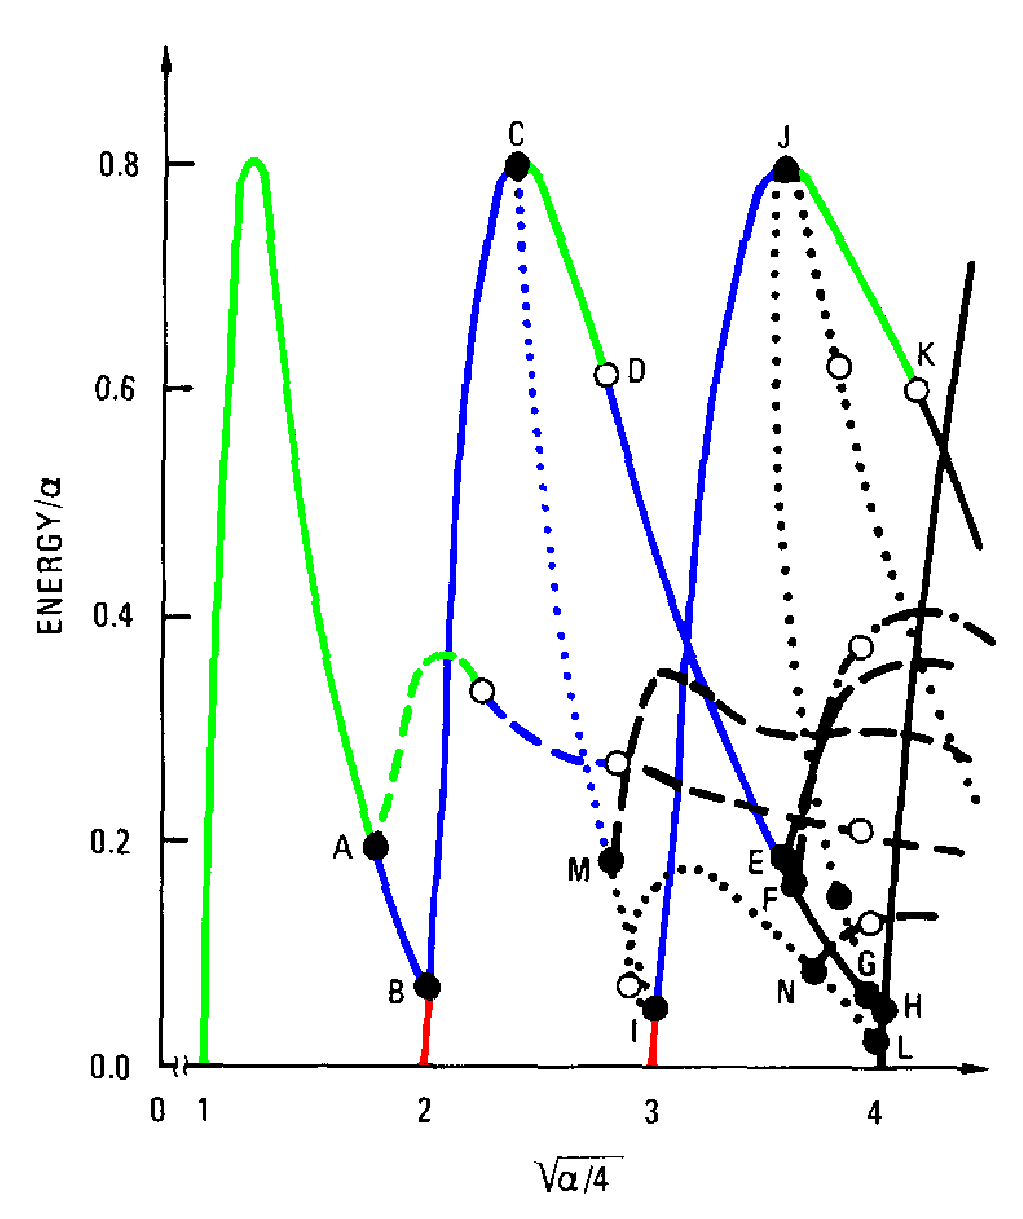
\includegraphics[width=0.5\textwidth]{figs/GreeneKimBifColor.eps}
	% \vspace*{-5pt}
\caption{
	{\small
The ``energy'' of \eqva\ as a function of the bifurcation
parameter $\tildeL=\sqrt{\alpha}/2$, from \refref{ksgreene88}.
The solid curves denote $N$-cell solutions,
dotted curves GLMRT, the dash-dotted curve the
giant states, and dashed curves the propagating solutions.
Open circles indicate Hopf bifurcations. 
We have color-coded the branches to reflect the number of unstable
eigenvalues (or complex pairs). Red: 2 unstable eigenvalues, Blue: 1
unstable eigenvalue, Green: stable. Solutions not 
resolved in \refref{ksgreene88} or of no interest
to our present purposes have been left black.
        } %end \small
        }
\label{fig:GreeneKim}
	% \vspace*{-5pt}
\end{figure}
%%%%%%%%%%%%%%%%%%%%%%%%%%%%%%%%%%%%%%%%%%%%%%%%%%%%%%%%%%%%%%%%%%

Greene and Kim study extends the earlier work\rf{Mks86,laquey74}
on the \KS\ \eqva\ and their bifurcations. The 
bifurcation diagram \reffig{fig:GreeneKim} summarizes the results
relevant to the system sizes studied here. 
\PC{
Please redraw bifurcation diagram \reffig{fig:GreeneKim} from the 
scratch in xfig (that will make it easier for me to edit), labeling
the axes with our symbols, and various \eqva\ with our - still in flux -
notation for them. Indicate also by circles the nature of
bifurcations for $u(x) = 0$ \eqv. I though those were Hopf? Wrong?
For the thesis, make schematic plots of each bifurcation, 
in style of Strogatz or whatever standard textbook on bifurcations
you like the best. You will help Jonathan and me understand what precisely
these bifurcations are. Thanks!
	}
\PC{indicate Christiansen at al. and Lan and Cvitanovi\'c  choices of 
    system size on the $\tildeL$ axis
    in \reffig{fig:GreeneKim}. Might require thinking - they are
    in the antisymmetric subspace, I tend to 1/2 them but here one should
    not.}

For small $\alpha$ the only \eqv\ of the system is the constant solution $y(x,t)=0$,
which is globally attracting 
for $\tildeL=\sqrt{\alpha}/2<1$. At $\tildeL=N$, with $N$ integer, 
the $N$th harmonic becomes unstable and the constant solution
bifurcates to the so called $N$-cell states. 
These states contain only the multiples of the $N$th
harmonic, {\ie} only the components $a_N,a_{2N},...$ in our notation. 
Moreover, the $N$-cell states are found to be symmetric (in our case, since $u=y_x$ they will be
antisymmetric). 
Greene and Kim show that symmetric solutions are \eqva, not \reqva. 
At point $A$ in \reffig{fig:GreeneKim} the $1$-cell state loses stability
and bifurcates to a stable, 
asymmetric \reqv, which later on becomes unstable through a Hopf bifurcation. 
\PC{harmonize our notation with the ``$N$-cell state" notation}

At $\tildeL=2$ the system has become large enough that a $2$-cell \eqv\ appears. At point $B$
in \reffig{fig:GreeneKim} the $1$-cell branch merges to the $2$-cell branch. In general each $N$-cell branch merges to the corresponding $2N$-cell branch.

At point $C$ in \reffig{fig:GreeneKim} the $2$-cell state bifurcates to a type of 
\eqv\ solution
found by La Quey, Mahajan, Rutherford and Tang\rf{laquey74} and generalized by Greene and Kim who refer to them as GLMRT \eqva. GLMRT solutions are symmetric 
($u(x)$ is antisymmetric)
and can be roughly described as long-wave distorted $N$-cell states.

The last type of solution identified in \refref{ksgreene88} appears at point $F$ 
in \reffig{fig:GreeneKim} and is called a
``giant" state because its amplitude grows as the system size increases.

According to the bifurcation diagram \reffig{fig:GreeneKim}, 
at the point that corresponds to system size $\tildeL=\alpha^{1/2}/2=3.501$
studied here,
the {\eqva} we expect are the $2$- and $3$-cell states ($\EQV{2}$ and $\EQV{3}$ respectivelly), the GLMRT state that bifurcates from a $3$-cell state at point $I$ ($\EQV{1}$),
the \reqva\ that belong to the branches starting at points $A$ ($\REQV{\pm}{1}$),
and $M$ that we have not  yet identified.
 
